\documentclass[final,20pt]{beamer}

% To change orientation of poster (landscape/portrait), adjust line 13 in _template.tex
% Gemini theme
% https://github.com/anishathalye/gemini


% ====================
% Packages
% ====================

\usepackage[T1]{fontenc}
\usepackage{lmodern}
\usepackage[orientation=landscape,size=a1,scale=1.3]{beamerposter}
\usetheme{gemini}
\usecolortheme{tudelft}

\usepackage{graphicx}
\usepackage{booktabs}
\usepackage{siunitx}
\usepackage{amsmath}
\usepackage{physics}
\usepackage{tikz}
\usepackage{pgfplots}
\pgfplotsset{compat=1.14}
\usepackage{anyfontsize}
\usepackage[
    bibencoding=utf8,
	url=false,
    doi=false,
	style=ieee,
    citestyle=numeric-comp,
    maxcitenames=2,
]{biblatex}
\usepackage[labelfont=bf]{caption}
\usepackage{hyperref}
\usepackage[capitalize,noabbrev,nameinlink]{cleveref}

\DeclareGraphicsRule{.ai}{pdf}{.ai}{}

\hypersetup{
    colorlinks=true,
    allcolors=cyan,
}
\urlstyle{same}

\let\chyperref\cref
\renewcommand{\cref}[1]{\hyperlink{#1}{\chyperref{#1}}} 


% ====================
% Lengths
% ====================

% If you have N columns, choose \sepwidth and \colwidth such that
% (N+1)*\sepwidth + N*\colwidth = \paperwidth
\newlength{\sepwidth}
\newlength{\colwidth}
\setlength{\sepwidth}{0.025\paperwidth}
\setlength{\colwidth}{0.3\paperwidth}

\newcommand{\separatorcolumn}{\begin{column}{\sepwidth}\end{column}}

\setlength{\leftmargini}{12mm}

\renewcommand*{\bibfont}{\footnotesize}

\setlength{\biblabelsep}{0.3\labelsep}


% ====================
% Logo
% ====================

% use this to include logos on the left and/or right side of the header:
\logoright{
\includegraphics[width=11cm]{logo_tudelft.pdf}}
\logoleft{
\includegraphics[width=8.5cm]{logo_hpd.png}}


% ====================
% Header
% ====================

\institute[shortinst]{Faculty of Aerospace Engineering, TU Delft, Netherlands}


\title{High-accuracy radiation pressure models \\ for the Lunar Reconnaissance Orbiter}
\author{Dominik Stiller (B.Sc. student) \and Advised by Dr. Dominic Dirkx}


\footercontent{
  \href{https://github.com/DominikStiller}{\color{white}{https://github.com/DominikStiller/hpb-project}} \hfill
  Honours Programme Bachelor of the Faculty of Aerospace Engineering --- Symposium 2023\hfill
  \href{mailto:d.stiller@student.tudelft.nl}{\color{white}{d.stiller@student.tudelft.nl}}}
  
\addbibresource{../references/bibliography.bib}


\begin{document}

\begin{frame}[t]
\begin{columns}[t]
\separatorcolumn

\begin{column}{\colwidth}

  \begin{exampleblock}{Abstract}

    Centimeter-scale orbit determination is necessary for satellite navigation and spaceborne geodesy. Orbits are sensitive to perturbations such as radiation pressure (RP) due to solar radiation as well as planetary albedo and thermal emissions. This project investigated sensitivities of orbit predictions to varying complexity in RP models for the Lunar Reconnaissance Orbiter (LRO) at $\beta \approx \ang{0}$. We found that solar RP dominates but lunar RP affects secular variations in semi-major axis and argument of periapsis. A constant-albedo lunar model and a paneled LRO model are recommended for precise radial and along-track positioning.

  \end{exampleblock}


  \begin{block}{Background}

    LRO was launched in June 2009 and mapped the Moon from a polar orbit at 50 km altitude~\cite{Tooley2010}. To exploit the accuracy of its laser altimeter, errors of at most 50--100 m (total) and 1 m (radial) are required. Even minor dynamic mismodeling impacts altimetry data reduction and may bias scientific interpretation. Understanding the effect of RP modeling choices on LRO's orbit can contribute to a more robust error budget of orbit determination results.

    The models from this work were integrated into and results were obtained with the TU Delft Astrodynamics Toolbox (\url{http://tudat.tudelft.nl/}). They will be used for future research and education activities at TU Delft.

  \end{block}

  \begin{block}{Source and target models}

    \begin{itemize}
      \item Sun: Point source with position from ephemeris.
      \item Moon: Discretized into 70 000 uniform panels (\geq 770 visible). Albedo distribution can vary spatially due to a low-resolution spherical harmonics expansion (DLAM-1~\cite{Floberghagen1999}) or constant (with DLAM-1 mean). Thermal emissions are based on the spacecraft--subsolar point angle.
      \item LRO: Can be paneled (10 panels, SA tracks Sun) or a "cannonball" (sphere of paneled-equivalent cross section with fixed reflectivity). % The bus attitude is based on definitive ephemerides.
    \end{itemize}

    \begin{figure}[b]
      \centering
      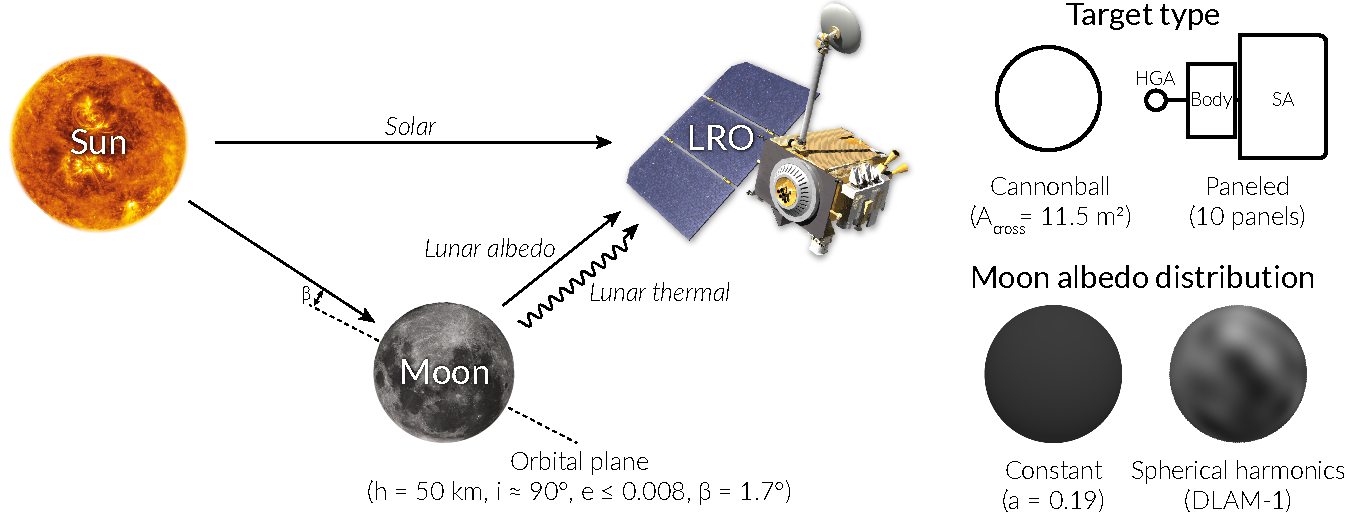
\includegraphics[width=\linewidth]{models.pdf}
      \caption{RP components and their models of varying complexity.}
      \label{fig:models}
    \end{figure}

  \end{block}

\end{column}

\separatorcolumn

\begin{column}{\colwidth}

  \begin{block}{Results: Radiation pressure acceleration}

    We predicted a 2.5-day arc (32 revolutions) with ephemeris-based initial conditions such that $\beta = \ang{1.7}$, i.e., LRO crosses above the subsolar point. RP accelerations due to Sun ($\vb a_\text{sun}$) and Moon ($\vb a_\text{moon}$) are shown in \cref{fig:acc}. Noteworthy observations:
    \begin{itemize}
      \item Radial RP: The radial components (top row) dominate, particularly above the subsolar point. Since they oppose each other, considering lunar RP dampens periodic change in radial position (\cref{fig:error}).
      \item Along-track RP: The along-track component of $\vb a_\text{sun}$ (middle row) is large away from but symmetric about the subsolar point. This leads to along-track drift, which changes the argument of periapsis (\cref{fig:kepler}).
      \item Along-track and cross-track components of $\vb a_\text{moon}$ have opposite signs for cannonball and paneled target models.
      \item All accelerations vanish in the eclipse region, including thermal. The Sun is occulted for 42\% of the orbit (47 min out of 113 min).
      \item A paneled target model allows more nuance over an orbit, e.g., due to solar panel pointing; there is no single equivalent cannonball model.
    \end{itemize}

    \begin{figure}[h]
      \centering
      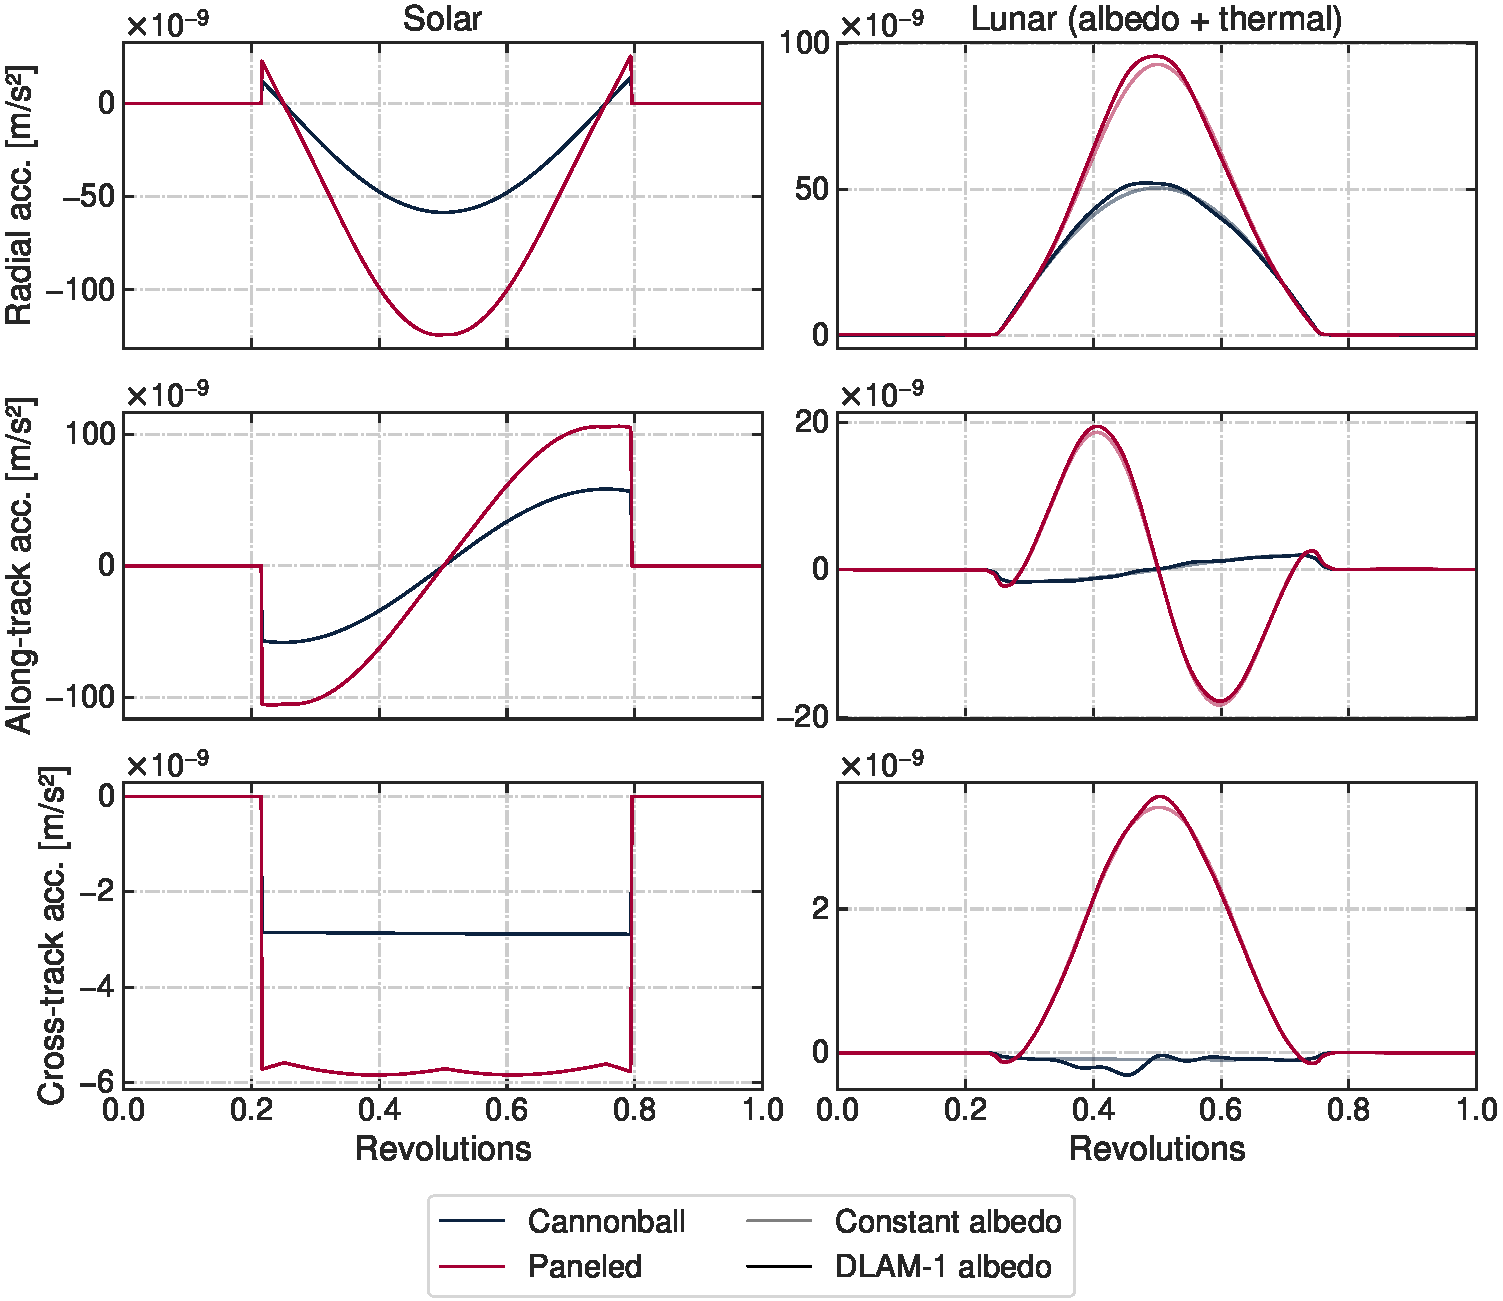
\includegraphics[width=\linewidth]{../analysis/plots/poster/rp_acceleration.pdf}
      \caption{RP accelerations due to Sun and Moon. Note the different y-axis scales.}
      \label{fig:acc}
    \end{figure}
    % TODO increase height if space permits

  \end{block}

\end{column}

\separatorcolumn

\begin{column}{\colwidth}

  \begin{alertblock}{Results: Change in orbit}

    \begin{figure}[h]
      \centering
      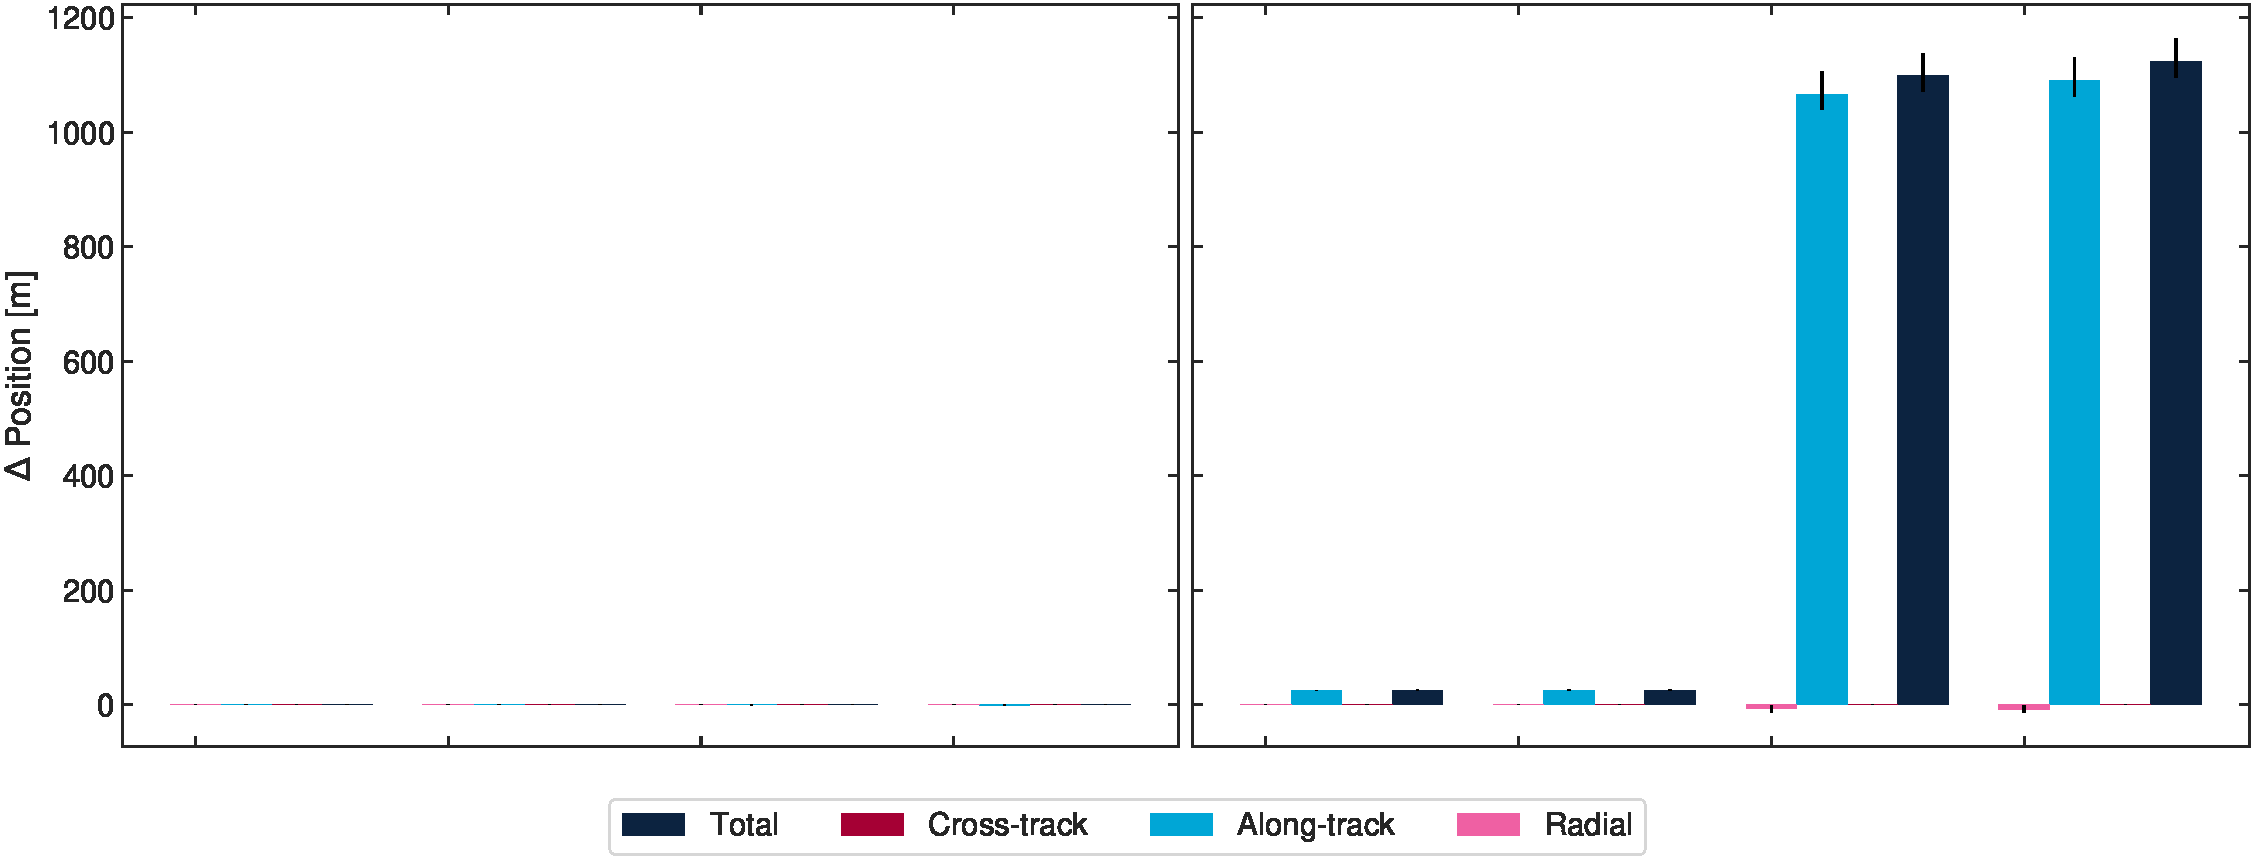
\includegraphics[width=\linewidth]{../analysis/plots/poster/final_position_error.pdf}
      \caption{Difference in position w.r.t. baseline (no RP) after 2.5 days. Results are invariant with albedo distribution. The secular radial error for a paneled target is below 20 cm but varies periodically up to 14 m. The cross-track difference is negligible. }
      \label{fig:error}
    \end{figure}
    \begin{figure}[h]
      \centering
      \includegraphics[width=\linewidth]{../analysis/plots/poster/kepler_elements_final.pdf}
      \caption{Change in mean orbital elements w.r.t. baseline after 2.5 days. Lunar RP increases the semi-major axis change but reduces the argument of periapsis change.}
      \label{fig:kepler}
    \end{figure}

  \end{alertblock}

  \begin{block}{Conclusion}

    \begin{itemize}
      \item Solar RP is the largest contributor; lunar RP particularly affects the semi-major axis and argument of periapsis.
      \item Since the exposed cross section changes over an orbit, a cannonball model with fixed properties is inappropriate for complex spacecraft.
      \item The choice of constant albedo or DLAM-1 does not influence RP accelerations, likely since thermal lunar radiation dominates.
      \item Solar RP has virtually no computational overhead, but high-resolution lunar paneling increases the walltime duration elevenfold; a paneled target only has overhead in conjunction with a paneled source.
    \end{itemize}


  \end{block}
  

  \begin{block}{References}

    \footnotesize{\printbibliography}

  \end{block}

\end{column}

\separatorcolumn
\end{columns}
\end{frame}

\end{document}
